\documentclass[10pt]{article}

\usepackage[margin=1in]{geometry}
\usepackage{amsmath,amssymb}
\usepackage{booktabs}
\usepackage{array}
\usepackage{pgfplots}
\usepackage{hyperref}
\usepackage{url}
\pgfplotsset{compat=1.18}

\title{Sparse Carried-State TTT for V-JEPA 2.1}
\author{Burn JEPA Contributors}
\date{Preprint draft, May 2026}

\begin{document}
\maketitle

\begin{abstract}
V-JEPA 2.1 produces dense video features with a tubelet encoder, but dense
patchification and dense token processing are a poor fit for streaming systems
whose visible regions are already sparse.  We present a Burn-native sparse
V-JEPA 2.1 implementation and an encoder-only training recipe, Sparse
Carried-State TTT (SC-TTT), that carries recurrent fast weights across adjacent
video windows while retaining deployable free-run inference semantics.  This is
an empirical systems contribution, not a claim of theoretical originality or
state-of-the-art video representation learning.  The implementation maps all
312 tensors from the official \texttt{vjepa2\_1\_vit\_base\_384} checkpoint and
matches the upstream \texttt{torch.hub} sparse encoder/predictor to
$2.92\times 10^{-5}$ max absolute error.  A verified SC-TTT checkpoint trained
with packed-stream TBPTT, sparse context rollout, dense stabilization samples,
state decay, state/update regularization, and a low-weight LeJEPA-style latent
Gaussian regularizer achieves sparse free-run loss/cosine $0.3209/0.8674$ over
the 164-window held-out manifest, improving over a base sparse V-JEPA 2.1 lane
at $0.4273/0.8187$ and over a reset-each-window trained-adapter lane at
$0.3990/0.8309$.  That manifest alone is too short for a long-run stability
claim: its longest contiguous stream is only 33 windows.  We therefore add
explicit repeated-stream, scene-stitch, and adversarial-stitch stress gates.
Those gates show that unbounded carried state is not stable: same-stream
carry over 136 windows drifts by $+0.1772$ loss and forced scene stitching
drifts by $+0.2124$ loss without resets.  A long-stable continuation with
periodic reset every 16 windows and scene-change reset recovers: the repeated
same-stream gate has near-zero late--early drift ($+0.0049$ loss over 136
windows), scene stitching improves after switches, and adversarial stitching
remains bounded by resetting on every detected scene switch.  The claim is
therefore bounded-horizon arbitrary-duration operation under an explicit
reset/decay policy, not unlimited memory carry.  The main remaining gates are
larger open-set video, repeated measurements, downstream baselines, and
lower-cost backward/optimizer kernels.
\end{abstract}

\section{Introduction}

V-JEPA 2.1 is a joint-embedding predictive architecture for image and video
self-supervision \cite{mur2026vjepa21}.  Its video path is naturally dense: for
a 16-frame 256px clip with 16px patches and tubelet size 2, the encoder sees
2048 video tokens before masking.  Streaming perception pipelines often know
that only a subset of image regions should be refreshed, for example from
AutoGaze or patch-difference attention.  The question in this paper is whether
V-JEPA 2.1 can use those sparse regions directly while retaining some of the
temporal information normally supplied by dense video tubelets.

We study this as a systems and distillation problem.  The contribution is a
measured implementation and training protocol: Burn-native V-JEPA 2.1 parity,
sparse positional indexing, sparse GPU patchification, sparse encoder-side TTT
rollout, stream-aware TBPTT training, and diagnostics that separate deployable
free-run behavior from teacher-forced or dense diagnostic paths.  We do not
claim that the method is theoretically original, the first sparse V-JEPA
system, or state of the art.  The current evidence is strong enough to support
a reproducible engineering method and a research agenda; it is not yet a final
production model.

Recent LeJEPA and LeWorldModel work argues that JEPA training can be stabilized
by adding an explicit Gaussian latent regularizer instead of relying only on
EMA, stop-gradient, architectural priors, or multi-term loss stacks
\cite{balestriero2025lejepa,maes2026leworldmodel}.  Weak-SIGReg further
motivates covariance-sketch variants as a cheaper regularization surface
\cite{akbar2026weaksigreg}.  We adopt this direction conservatively: the
teacher remains the official pretrained V-JEPA 2.1 model, and the added term is
a small student-token stabilizer rather than a replacement for teacher
distillation.

\section{Problem Statement and Scope}

\paragraph{Problem statement.}
Let $V_i\in\mathbb{R}^{B\times C\times T\times H\times W}$ be the $i$-th
video window from a stream and let $G$ be the V-JEPA tubelet grid.  A sparse
context mask $M_i\subseteq G$ selects the tokens refreshed for that window.
Given a frozen dense V-JEPA teacher $E_\theta$, learn an encoder-only student
$S_\psi$ with recurrent TTT state $F_i$ such that
\begin{equation}
  S_\psi(V_i,M_i,F_{i-1}) \approx E_\theta(V_i)
\end{equation}
on the selected evaluation tokens, while avoiding dense patchification and
while updating $F_i$ without privileged teacher tokens at inference time.

\paragraph{Assumptions.}
The experiments and system design rely on the following assumptions.
\begin{enumerate}
\item The loaded checkpoint is the official V-JEPA 2.1 ViT-B checkpoint and
  sparse encoder/predictor parity is checked before quality claims.
\item Sparse masks are available before JEPA patchification.  They may come
  from AutoGaze, patch-difference logic, or precomputed manifests.
\item The deployed student updates TTT state from detached student hidden
  states.  Teacher-forced updates are diagnostics only.
\item Long-running streams use the trained reset/decay policy.  The current
  production policy resets carried TTT state every 16 windows and on scene
  changes.  Unbounded state carry is a measured failure case, not a supported
  deployment mode.
\item Feature distillation against the dense teacher is a proxy objective.  We
  do not yet report downstream task accuracy.
\item Frozen sparse-patchify training is the intended adapter-training bridge.
  Full unfrozen finetuning is a higher-risk ablation.
\end{enumerate}

When these assumptions are violated, the expected failure mode changes.  If
the mask misses semantic updates, the feature cache can become stale.  If state
is carried far beyond the trained horizon without reset or decay, fast weights
decohere in the repeated-stream stress gate.  If scene switches are stitched
without resetting the TTT state, the state contaminates the next scene.  If
dense diagnostic probes are enabled over large full-token tensors, the current
CUDA backend can exhaust allocator pages.

\section{Definitions and Formal Guardrail}

This section is included to make the evaluation terminology precise.  It is
not a claim that the paper is theoretically original.

\paragraph{Definition 1: Carried-state coherence gap.}
For an ordered stream dataset $\mathcal{D}=\{(V_i,M_i)\}_{i=1}^n$, let
$L_{\mathrm{run}}$ and $C_{\mathrm{run}}$ be the average feature loss and
cosine similarity of the deployable free-run student with persistent state
$F_i=U_\psi(F_{i-1},V_i,M_i)$.  For a diagnostic intervention $q$ such as
reset-each-frame, freeze-fast-update, shuffle, or reverse order, define
\begin{align}
  \Delta_L(q) &= L_q - L_{\mathrm{run}}, \\
  \Delta_C(q) &= C_{\mathrm{run}} - C_q.
\end{align}
Positive $\Delta_L(q)$ and $\Delta_C(q)$ mean that the persistent temporal
state is useful relative to intervention $q$.  Longitudinal drift is measured
by $L_{\mathrm{late}}-L_{\mathrm{early}}$ and
$C_{\mathrm{late}}-C_{\mathrm{early}}$ over ordered eval-window segments.
This refines an ordinary average eval loss by testing whether memory helps and
whether it remains stable through time.

\paragraph{Proposition 1: zero-output TTT insertion is initially
function-preserving.}
Assume a pretrained encoder block computes $X \mapsto B_\theta(X)$, and a TTT
adapter is inserted as a residual
\begin{equation}
  A_\psi(X,F) = X + W_o \phi_\psi(X,F),
\end{equation}
where $W_o=0$ at initialization.  Then the augmented block output equals the
pretrained block output for every input $X$ and fast state $F$ before training.

\paragraph{Proof.}
At initialization, $W_o=0$.  Therefore
\[
  A_\psi(X,F) = X + 0\cdot \phi_\psi(X,F) = X.
\]
Replacing the identity residual path before or after the pretrained block
therefore does not change the value passed to the rest of the encoder.  By
composition over all inserted adapters, the augmented encoder is identical to
the pretrained encoder before adapter training.  The argument assumes exact
zero initialization of the adapter output projection and identical positional
and token-order inputs; it does not prove anything about trained fast-state
stability.
\hfill$\square$

\section{Method: Sparse Carried-State TTT}

\subsection{Sparse V-JEPA Forward}

For context mask $M_c$ and target mask $M_t$, sparse V-JEPA computes
\begin{equation}
  z_c = E_\theta(V, M_c), \qquad \hat{z}_t = P_\theta(z_c, M_c, M_t).
\end{equation}
Sparse plans cache token indices, sequence order, coordinates, and positional
encoding tensors.  The CUDA and WGPU sparse-patchify paths use
\texttt{burn\_flex\_gmm} so masked pixels are skipped before patch embedding
instead of gathered after dense patchification.

\subsection{SC-TTT Adapter}

Each selected encoder layer receives a zero-output residual adapter with a fast
state $F$.  For hidden tokens $X$, the adapter reads memory with
\begin{equation}
  X + W_o(XF/\sqrt{d}),
\end{equation}
then updates $F$ from chunked, detached student hidden states.  The output
projection is zero-initialized, so the untrained adapter starts as a no-op by
Proposition 1.  We place TTT modules only in the encoder because the shipped
artifact is an encoder representation; predictor-side adapters would adapt a
training head and add work after sparse token extraction.

\subsection{Latent Stability Regularizer}

The selected run adds a low-weight LeJEPA/SIGReg-inspired penalty to the
student tokens used by the feature loss.  For aligned student tokens
$Z\in\mathbb{R}^{N\times d}$, the implemented regularizer is
\begin{equation}
R(Z) =
\lambda\left[
\alpha_\mu \|\mu(Z)\|_2^2 +
\alpha_\sigma \|\mathrm{var}(Z)-\mathbf{1}\|_2^2 +
\alpha_c C_{\mathrm{sketch}}(Z)
\right],
\end{equation}
where $C_{\mathrm{sketch}}$ is a deterministic adjacent-feature covariance
sketch over the first 64 feature dimensions.  The implementation is
device-resident and mask-aware; padded ragged tokens are excluded from the
mean/variance estimates.  This is not a full LeJEPA replacement objective: the
V-JEPA 2.1 teacher remains fixed, and the regularizer is used only as a small
anti-collapse/stability term for the student rollout.

\paragraph{Algorithm 1: Sparse Carried-State TTT (SC-TTT).}
\begin{enumerate}
\item Load the official V-JEPA 2.1 teacher and initialize an encoder student
  with zero-output TTT adapters at layers $[3,7,11]$.
\item For each packed stream batch, restore one fast state per stream key.
\item Resolve sparse context/target masks from the manifest or mask driver.
\item Run the frozen dense teacher on the full video window and detach the
  teacher features.
\item Roll the student through sparse frame/tubelet inputs, updating fast
  state from detached student hidden states.
\item Minimize feature MSE between student tokens and selected teacher tokens,
  optionally plus $R(Z)$.
\item Detach the carried fast state at the TBPTT boundary, apply decay, and
  store it under the stream key.
\item Periodically include dense stabilization samples and scheduled resets so
  the adapter learns both zero-state initialization and carried-state use.
\end{enumerate}

\section{Experimental Protocol}

All numerical correctness claims use the official
\texttt{vjepa2\_1\_vit\_base\_384} checkpoint loaded from Meta's V-JEPA 2.1
\texttt{torch.hub} entry point.  Quality runs use local open-set video windows
at 256px with 16-frame student clips and a frozen 3D teacher.  The verified
SC-TTT run uses sparse context masks with 410 of 2048 tokens (20.0\%) and 103
target tokens (5.0\%).

Long-rollout eval uses sequential manifest order with batch size 1 so state is
actually carried across adjacent windows.  Packed-stream eval is useful for
throughput, but round-robin stream packing can hide whether a single stream is
being carried continuously.  Diagnostic probes compare the deployable free-run
state against reset-each-frame, reset-each-tubelet, shuffle, reverse, and
freeze-fast-update interventions.

Backend labels are conservative.  Burn exposes both \texttt{webgpu} and
\texttt{wgpu} feature gates; they are related WebGPU-family lanes unless a row
specifically measures the native WGPU \texttt{burn\_flex\_gmm} extension.

\section{Results}

\subsection{Numerical Correctness}

\begin{table}[t]
\centering
\caption{V-JEPA 2.1 ViT-B parity against the official \texttt{torch.hub}
module.  Entries are max absolute error.}
\label{tab:parity}
\begin{tabular}{lccc}
\toprule
Case & Sparse encoder & Predictor & Target tokens \\
\midrule
Micro sparse 2x2 & $1.109{\times}10^{-5}$ & $1.812{\times}10^{-5}$ & $1.034{\times}10^{-5}$ \\
Multi-tubelet 3x4 & $1.335{\times}10^{-5}$ & $1.597{\times}10^{-5}$ & $2.921{\times}10^{-5}$ \\
\bottomrule
\end{tabular}
\end{table}

The loader applies all 312 mapped tensors with no missing, skipped, or errored
tensors.  The multi-tubelet case exercises temporal indexing, non-square
spatial position handling, sparse context gather, target gather, and predictor
ordering.

\subsection{Verified Checkpoint and Long-Rollout Coherence}

\begin{table}[t]
\centering
\caption{Verified checkpoints and rejected continuation.  The full-manifest
quality row uses \texttt{stage1-stream-tbptt-sigreg/ttt-model.mpk}; the
long-rollout stress gates select the continued
\texttt{stage1-stream-tbptt-longstable/ttt-model.mpk} checkpoint.}
\label{tab:verified}
\begin{tabular}{lrrrr}
\toprule
Run & Steps & Samples & Best train loss & Final sampled loss \\
\midrule
SC-TTT + SIGReg selected & 160 & 320 & 0.1829 & 0.3111 \\
SC-TTT long-stable continuation & 128 & 256 & 0.1653 & 0.2479 \\
SC-TTT unregularized & 160 & 320 & 0.1828 & 0.3111 \\
Low-LR continuation & 96 & 192 & 0.2555 & 0.2555 \\
\bottomrule
\end{tabular}
\end{table}

The SIGReg run exercises the intended training path: 211 carried windows, 109
reset windows, 320 detached/decayed states, and dense stabilization samples on
55 of 160 optimizer steps.  The long-stable continuation starts from SIGReg,
keeps the same encoder-only adapter placement, trains on repeated continuous
streams, and ends with a reset interval of 16 windows.  It contributes 184
carried windows, 72 reset windows, and 256 detached/decayed states.  The low-LR
continuation improved sampled training loss but is not selected because its
long-rollout eval worsened.

\begin{table}[t]
\centering
\scriptsize
\setlength{\tabcolsep}{3pt}
\caption{LeJEPA/SIGReg-style latent regularizer ablation.  The 64-step rows use
a matched 24-window held-out subset; the selected row is the full 160-step
checkpoint evaluated on the full 164-window sequential manifest.  The added
term is non-regressive but effectively neutral at this scale.}
\label{tab:sigreg}
\begin{tabular}{lrrrrr}
\toprule
Run & Reg weight & Eval samples & Feature loss & Cosine & Reg loss \\
\midrule
64-step off & 0 & 24 & 0.3478696 & 0.8516861 & -- \\
64-step low & 1e-5 & 24 & 0.3478668 & 0.8516874 & 5.82e-6 \\
64-step high & 5e-5 & 24 & 0.3478670 & 0.8516872 & 2.91e-5 \\
160-step selected & 1e-5 & 164 & 0.3208972 & 0.8674483 & 6.19e-6 \\
\bottomrule
\end{tabular}
\end{table}

\begin{table}[t]
\centering
\caption{Short sequential carried-state eval.  These rows use free-run student
state, not teacher-forced adapter updates.}
\label{tab:coherence}
\begin{tabular}{lrrrr}
\toprule
Eval & Samples & Carried/reset & Loss & Cosine \\
\midrule
Sparse SC-TTT selected & 24 & 21 / 3 & 0.3334 & 0.8629 \\
Sparse low-LR continuation & 24 & 21 / 3 & 0.3977 & 0.8410 \\
Dense selected & 16 & 15 / 1 & 0.3946 & 0.8448 \\
\bottomrule
\end{tabular}
\end{table}

\begin{table}[t]
\centering
\scriptsize
\setlength{\tabcolsep}{3pt}
\caption{Full held-out manifest sparse ablation.  The base sparse row is
V-JEPA 2.1 with the same sparse context masks and zero-output TTT insertion,
which is function-preserving before adapter training.  The manifest has 164
windows across 19 streams; the longest contiguous stream is 33 windows.}
\label{tab:longitudinal}
\begin{tabular}{lrrrrrr}
\toprule
Eval & Samples & Carry/reset & Longest & Loss & Cosine & Late--early loss \\
\midrule
V-JEPA 2.1 sparse & 164 & 145 / 19 & 33 & 0.4273466 & 0.8187255 & +0.0405 \\
SC-TTT + SIGReg sparse & 164 & 145 / 19 & 33 & 0.3208972 & 0.8674483 & +0.0838 \\
SC-TTT sparse unregularized & 164 & 145 / 19 & 33 & 0.3208981 & 0.8674482 & +0.0838 \\
SC-TTT reset each window & 164 & 0 / 164 & 33 & 0.3989558 & 0.8308782 & +0.0417 \\
\bottomrule
\end{tabular}
\end{table}

\begin{table}[t]
\centering
\scriptsize
\setlength{\tabcolsep}{3pt}
\caption{Long-rollout stress gates added after the full manifest revealed that
33 contiguous windows were insufficient evidence.  No-reset rows are diagnostic
failures of unbounded carried state; reset-16 and scene-reset rows use the
long-stable continuation.  Lower late--early loss is better.}
\label{tab:stress}
\begin{tabular}{lrrrrr}
\toprule
Gate & Windows & Switches & Resets & Loss/cosine & Late--early loss \\
\midrule
Same stream, no reset & 136 & 0 & 1 & 0.4982 / 0.8046 & +0.1772 \\
Same stream, reset32 & 68 & 0 & 3 & 0.3720 / 0.8510 & +0.0837 \\
Same stream, reset16 & 136 & 0 & 9 & 0.3270 / 0.8666 & +0.0049 \\
Scene stitch, no scene reset & 64 & 10 & 1 & 0.4468 / 0.8218 & +0.2124 \\
Scene stitch, scene reset & 64 & 10 & 11 & 0.2896 / 0.8783 & -0.0675 \\
Adversarial stitch, scene reset & 64 & 63 & 64 & 0.4209 / 0.8215 & -0.0338 \\
\bottomrule
\end{tabular}
\end{table}

\begin{table}[t]
\centering
\caption{Carried-state coherence interventions for the selected sparse
checkpoint.  Positive loss gaps mean the persistent state is better.}
\label{tab:interventions}
\begin{tabular}{lcc}
\toprule
Intervention & Loss / cosine & Coherence gap vs. free-run loss \\
\midrule
Free-run persistent state & 0.3334 / 0.8629 & 0.0000 \\
Reset each frame & 0.4639 / 0.8047 & +0.1305 \\
Reset each tubelet & 0.4577 / 0.8074 & +0.1243 \\
Freeze fast updates & 0.4639 / 0.8047 & +0.1305 \\
Shuffle order & 0.4503 / 0.8106 & +0.1169 \\
Reverse order & 0.5894 / 0.7520 & +0.2560 \\
\bottomrule
\end{tabular}
\end{table}

Tables~\ref{tab:coherence}--\ref{tab:stress} are the current long-rollout
gate.  The selected checkpoint is coherent under the short diagnostic gate:
persistent memory is better than resetting, freezing, shuffling, or reversing
temporal order.  The full-manifest gate adds the direct V-JEPA 2.1+sparse
versus V-JEPA 2.1+SC-TTT+sparse ablation.  SC-TTT improves over base sparse by
$0.1064$ loss and $0.0487$ cosine, and over reset-each-window by $0.0781$ loss
and $0.0366$ cosine.  The SIGReg-style regularizer is a safe hook but does not
materially change the full-manifest result: feature loss shifts from
$0.3208981$ to $0.3208972$.

The stress gate is deliberately less favorable.  It repeats one stream beyond
the observed held-out horizon, stitches unrelated streams into one artificial
state trajectory, and alternates scenes adversarially.  The result is the
central limitation and the central fix: unbounded carried state fails, while a
bounded reset-16 policy and scene-change reset recover.  We therefore describe
SC-TTT as stable for arbitrary-duration processing under the explicit
reset/decay policy, not as a model with unlimited fast-memory lifetime.

\subsection{Mask Policies}

\begin{table}[t]
\centering
\caption{Representative 224px mask ablation at matched 20\% context density
from earlier controlled runs.  TTT improves all listed policies in that run,
but AutoGaze and patch-diff are close in quality.}
\label{tab:masks}
\begin{tabular}{lcccc}
\toprule
Mask policy & Single loss & TTT loss & Single cosine & TTT cosine \\
\midrule
Full-frame holdout & 0.1925 & 0.1729 & 0.9190 & 0.9274 \\
Random sparse & 0.2181 & 0.1960 & 0.9078 & 0.9173 \\
Patch-diff sparse & 0.1962 & 0.1798 & 0.9163 & 0.9235 \\
AutoGaze-style sparse & 0.1970 & 0.1803 & 0.9165 & 0.9238 \\
\bottomrule
\end{tabular}
\end{table}

This table does not justify a universal AutoGaze-is-best claim.  At matched
density, AutoGaze-style and patch-diff masks are close on teacher-feature
quality.  AutoGaze's practical advantage in the current pipeline is that
precomputed masks avoid patch-diff scoring and selection overhead.

\subsection{Throughput}

\begin{table}[t]
\centering
\caption{Representative AutoGaze-to-sparse-JEPA rolling throughput.}
\label{tab:e2e}
\begin{tabular}{llrrr}
\toprule
Lane & Resolution/density & Context tokens & Rolling ms & Rolling windows/s \\
\midrule
ndarray CPU & 224px / 1\% & 4 & 12.216 & 163.72 \\
WebGPU-family & 224px / 1\% & 4 & 33.824 & 59.13 \\
CUDA & 224px / 1\% & 4 & 3.918 & 510.41 \\
CUDA & 224px / 5\% & 20 & 6.769 & 295.46 \\
CUDA & 720p / 1\% & 72 & 3.937 & 507.99 \\
CUDA & 720p / 25\% & 1800 & 22.112 & 90.45 \\
\bottomrule
\end{tabular}
\end{table}

The CUDA sparse-patchify lane is the intended inference path.  WebGPU-family
throughput can be lower than CPU ndarray in low-density E2E rows because the
AutoGaze/mask side performs many short launches and synchronization points; it
is not evidence that dense CPU JEPA is faster than device-resident sparse GPU
JEPA.

\begin{figure}[t]
\centering
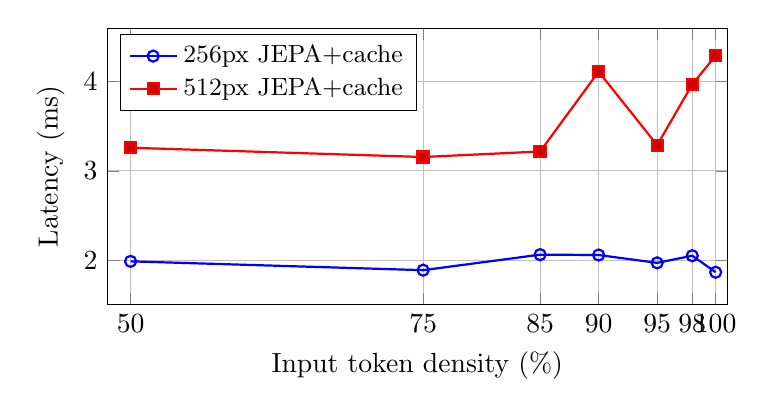
\begin{tikzpicture}
\begin{axis}[
    width=0.78\linewidth,
    height=0.42\linewidth,
    xlabel={Input token density (\%)},
    ylabel={Latency (ms)},
    xmin=48, xmax=101,
    ymin=1.5, ymax=4.6,
    xtick={50,75,85,90,95,98,100},
    grid=both,
    legend style={at={(0.02,0.98)},anchor=north west,font=\small},
]
\addplot+[mark=o,thick] coordinates {
    (50,1.986) (75,1.887) (85,2.061) (90,2.057)
    (95,1.969) (98,2.049) (100,1.864)
};
\addlegendentry{256px JEPA+cache}
\addplot+[mark=square*,thick] coordinates {
    (50,3.260) (75,3.156) (85,3.218) (90,4.113)
    (95,3.289) (98,3.970) (100,4.292)
};
\addlegendentry{512px JEPA+cache}
\end{axis}
\end{tikzpicture}
\caption{WGPU sparsity-latency sweep for the Bevy-style tiny JEPA+feature-cache
path.  The 100\% point is the dense ordered baseline.}
\label{fig:sparsity-latency}
\end{figure}

\begin{table}[t]
\centering
\caption{TTT forward+backward training-step sparsity sweep, batch 4.}
\label{tab:train}
\begin{tabular}{lrrr}
\toprule
Lane & 10\% sparse & 100\% dense & Gain \\
\midrule
WebGPU-family dense-patch path & 15.504 ms & 22.696 ms & 31.7\% \\
WGPU flex-gmm pixel-skip path & 8.790 ms & 13.957 ms & 37.0\% \\
CUDA dense-patch path & 14.627 ms & 20.809 ms & 29.7\% \\
CUDA flex-gmm pixel-skip path & 15.085 ms & 19.835 ms & 23.9\% \\
\bottomrule
\end{tabular}
\end{table}

Training speedups are not proportional to token reduction.  Adapter backward,
AdamW, transformer dispatch, and fixed kernel overhead remain in the timed
loop.  In the selected checkpoint run, backward plus optimizer consumed
414.7 s of 489.7 s train elapsed.

\section{Failure Cases and Limitations}

The evaluation includes cases where the method loses or the system fails.
First, the low-LR continuation improves sampled train loss but worsens sparse
carried eval from $0.3334/0.8629$ to $0.3977/0.8410$, so train loss alone is
not a sufficient model-selection criterion.  Second, the LeJEPA/SIGReg-style
regularizer is non-regressive but only neutral on the current V-JEPA 2.1
distillation run; it should be treated as a stability hook, not as evidence
that Gaussian regularization solves long-rollout drift here.  Third, unbounded
TTT state carry is a measured failure: the repeated same-stream gate drifts by
$+0.1772$ loss over 136 windows, and the stitched-scene gate drifts by
$+0.2124$ loss without scene reset.  Fourth, dense full-grid temporal
diagnostics over large token tensors currently hit a CubeCL CUDA allocator
panic; dense primary eval works, but dense diagnostic probes need chunking or
streaming.  Fifth, the 164-window held-out manifest check improves with
persistent state on average but has only 33 contiguous windows in one stream,
so it was insufficient by itself.  Sixth, patch-diff masks can miss slow
semantic changes; refresh policies such as age-priority, blue-noise refresh, or
keyframes are required for persistent feature caches.

The largest current quality run is still small compared with open-set video
pretraining.  The paper reports teacher-feature distillation metrics rather
than downstream task accuracy.  Results are mostly single-run measurements;
larger repeated sweeps are needed before claiming robustness or generality.

\section{Research Claim Audit}

Table~\ref{tab:audit} applies the research contribution checklist directly.
The correct classification is a measured systems method with an algorithmic
recipe.  It should not be described as theoretically original.  It should also
avoid the phrase ``novel algorithm'' until broader external baselines,
repeated statistics, and downstream task results are available.

\begin{table}[t]
\centering
\scriptsize
\setlength{\tabcolsep}{3pt}
\caption{Minimum evidence table for contribution wording.}
\label{tab:audit}
\begin{tabular}{@{}p{0.22\linewidth}p{0.28\linewidth}p{0.08\linewidth}p{0.32\linewidth}@{}}
\toprule
Claim type & Required evidence & Present? & Notes \\
\midrule
Theoretical originality & New definition & partial & Definition 1 names a useful coherence metric, but it is evaluative rather than a central new theory. \\
Theoretical originality & Theorem/proposition & partial & Proposition 1 is a correctness guard for zero-init adapters, not a deep theory result. \\
Theoretical originality & Checkable proof & yes & Included for Proposition 1. \\
Theoretical originality & Assumptions & yes & Listed in Section 2. \\
Theoretical originality & Minimal implementation & yes & SC-TTT maps directly to the encoder adapter path. \\
Theoretical originality & Benchmark where method can lose & yes & Low-LR continuation and dense diagnostic failure. \\
Theoretical originality & Failure case & yes & Section 8. \\
Novel algorithm & Baseline & yes & Base sparse V-JEPA 2.1, reset, freeze, reverse/shuffle, dense, low-LR continuation, zero/no-op insertion. \\
Novel algorithm & Measurable improvement & yes & SC-TTT sparse beats base sparse V-JEPA by 0.1064 loss and reset-each-window by 0.0781 loss on the full manifest. \\
Novel algorithm & Ablation & yes & State reset, freeze, order, mask, density, backend, continuation, latent regularizer. \\
Novel algorithm & Reason it works & partial & Memory-intervention gaps support the mechanism; more external validation is needed. \\
Novel algorithm & Case where it does not work & yes & Low-LR continuation, dense diagnostic allocator pressure, unbounded state carry, and unreset scene stitching. \\
Novel algorithm & Short memorable name & yes & Sparse Carried-State TTT (SC-TTT). \\
\bottomrule
\end{tabular}
\end{table}

\paragraph{Final gate answers.}
The new concept is the carried-state coherence gap for deployable sparse TTT
rollouts.  The formal claim is the zero-output adapter insertion proposition.
The proof is algebraic and only covers initialization.  The algorithmic recipe
is SC-TTT.  It beats base sparse V-JEPA 2.1 on the full 164-window manifest,
beats reset/freeze/order-intervention baselines on the short verified sparse
long-rollout eval, and beats reset-each-window on the 164-window held-out
manifest.  It fails when state is carried without reset beyond the trained
horizon or through unrelated scene switches.  It recovers when the deployment
policy resets every 16 windows and on scene changes.  Other failures occur
when train-loss-only continuation worsens carried eval, when the latent
Gaussian regularizer is only neutral, when diagnostic dense probes exceed
backend memory behavior, and when masks miss semantic updates.  Those failures
violate the assumptions that eval selection matches deployment, diagnostics
are chunked, sparse masks cover semantic changes, and the reset/decay policy is
active.  Future work should scale data, add external and downstream baselines,
repeat measurements, chunk dense diagnostics, and improve sparse TTT
backward/optimizer kernels.

\section{Reproducibility Notes}

Selected artifact:
\begin{verbatim}
target/burn-jepa-production-final-256/
  stage1-stream-tbptt-sigreg/ttt-model.mpk
  stage1-stream-tbptt-longstable/ttt-model.mpk
\end{verbatim}

Training command:
\begin{verbatim}
MODEL=target/burn-jepa-production-final-256/stage1-stream-tbptt-sigreg/ttt-model.mpk
cargo run --no-default-features --features cuda,sparse-patchify-cuda \
  --bin burn-jepa -- train-ttt \
  --config configs/production/vjepa21-ttt-stage1-stream-tbptt-sigreg-cuda.toml

cargo run --no-default-features --features cuda,sparse-patchify-cuda \
  --bin burn-jepa -- train-ttt \
  --config configs/production/vjepa21-ttt-stage1-stream-tbptt-longstable-cuda.toml
\end{verbatim}

Sparse long-rollout eval:
\begin{verbatim}
MODEL=target/burn-jepa-production-final-256/stage1-stream-tbptt-sigreg/ttt-model.mpk
cargo run --no-default-features --features cuda,sparse-patchify-cuda \
  --bin burn-jepa -- eval-ttt \
  --config configs/production/vjepa21-ttt-long-rollout-sigreg-cuda.toml \
  --model "$MODEL" \
  --steps 164 --batch-size 1 --no-full-grid
\end{verbatim}

Full held-out manifest sparse ablation:
\begin{verbatim}
MODEL=target/burn-jepa-production-final-256/stage1-stream-tbptt-sigreg/ttt-model.mpk
cargo run --no-default-features --features cuda,sparse-patchify-cuda \
  --bin burn-jepa -- eval-ttt \
  --config configs/production/vjepa21-base-sparse-long-rollout-verylong-cuda.toml \
  --base-sparse \
  --steps 164

cargo run --no-default-features --features cuda,sparse-patchify-cuda \
  --bin burn-jepa -- eval-ttt \
  --config configs/production/vjepa21-ttt-long-rollout-sigreg-cuda.toml \
  --model "$MODEL" \
  --steps 164

cargo run --no-default-features --features cuda,sparse-patchify-cuda \
  --bin burn-jepa -- eval-ttt \
  --config configs/production/vjepa21-ttt-long-rollout-reset-window-cuda.toml \
  --model "$MODEL" \
  --steps 164
\end{verbatim}

Long-rollout stress gates:
\begin{verbatim}
LONG=target/burn-jepa-production-final-256/stage1-stream-tbptt-longstable/ttt-model.mpk
cargo run --no-default-features --features cuda,sparse-patchify-cuda \
  --bin burn-jepa -- eval-ttt \
  --config configs/production/vjepa21-ttt-long-rollout-cactus-repeat-reset16-cuda.toml \
  --model "$LONG" \
  --steps 136 --batch-size 1 --no-full-grid

cargo run --no-default-features --features cuda,sparse-patchify-cuda \
  --bin burn-jepa -- eval-ttt \
  --config configs/production/vjepa21-ttt-long-rollout-stitched-reset-4x-cuda.toml \
  --model "$LONG" \
  --steps 64 --batch-size 1 --no-full-grid

cargo run --no-default-features --features cuda,sparse-patchify-cuda \
  --bin burn-jepa -- eval-ttt \
  --config configs/production/vjepa21-ttt-long-rollout-adversarial-stitch-reset-4x-cuda.toml \
  --model "$LONG" \
  --steps 64 --batch-size 1 --no-full-grid
\end{verbatim}

Dense carried eval:
\begin{verbatim}
MODEL=target/burn-jepa-production-final-256/stage1-stream-tbptt-sigreg/ttt-model.mpk
cargo run --no-default-features --features cuda,sparse-patchify-cuda \
  --bin burn-jepa -- eval-ttt \
  --config configs/production/vjepa21-ttt-long-rollout-dense-eval-cuda.toml \
  --model "$MODEL" \
  --steps 16
\end{verbatim}

\section{Final Inference Performance Appendix}

Table~\ref{tab:gpu-util} reports native WGPU inference telemetry for the
deployed Bevy-style low-resolution feature pipeline.  The run used an NVIDIA
RTX PRO 6000 Blackwell Workstation Edition with driver 595.58.03.  Each row
loads the sharded V-JEPA 2.1 Burn package, runs four warmup frames, then
measures 48 synchronized low-resolution inference frames while sampling
\texttt{nvidia-smi} every 50 ms.  AnyUp and Bevy display-panel conversion are
disabled in this table so the measurement focuses on JEPA encode, sparse cache
update, and low-resolution PCA.  The sparse rows use a deterministic
patch-diff stream with 30\% cache-write density; the production
bucketed-context policy widens that to a 50\% encoder-token width to avoid
shape churn.  Sparse bucket prewarm is excluded from the timed frames.

\begin{table}[t]
\centering
\scriptsize
\caption{Final WGPU inference GPU-utilization appendix.  VRAM is peak absolute
device memory reported by NVML during the measured window; power and
utilization are mean NVML samples.}
\label{tab:gpu-util}
\begin{tabular}{llrrrrrrr}
\toprule
Model & Mode & Res. & Write/enc. & Mean ms & FPS & GPU util. & VRAM MiB & Power W \\
\midrule
Base & Dense & 256 & 100/100\% & 18.87 & 52.86 & 60.8\% & 1806 & 80.9 \\
Base & Dense & 512 & 100/100\% & 28.48 & 34.93 & 57.2\% & 3702 & 144.3 \\
Base & Sparse & 256 & 30/50\% & 20.40 & 48.91 & 68.0\% & 1958 & 80.0 \\
Base & Sparse & 512 & 30/50\% & 31.11 & 31.99 & 54.7\% & 3906 & 120.7 \\
SC-TTT & Dense & 256 & 100/100\% & 21.32 & 46.81 & 56.7\% & 2245 & 83.7 \\
SC-TTT & Dense & 512 & 100/100\% & 33.86 & 29.41 & 66.0\% & 3618 & 153.8 \\
SC-TTT & Sparse & 256 & 30/50\% & 21.63 & 46.15 & 56.2\% & 2247 & 88.3 \\
SC-TTT & Sparse & 512 & 30/50\% & 33.54 & 29.68 & 58.7\% & 3913 & 129.0 \\
\bottomrule
\end{tabular}
\end{table}

These measurements clarify two deployment caveats.  First, TTT adds modest
latency and memory at 256px and larger latency at 512px, as expected from the
adapter and carried-state work.  Second, WGPU sparse patchify is not a
guaranteed latency win at the default 30\% write / 50\% encode bucket.  At
this density, dense kernels remain highly competitive and sometimes faster;
the sparse WGPU path mainly reduces 512px power in these rows.  The larger
latency wins reported in Table~\ref{tab:e2e} still correspond to the CUDA
sparse-patchify lane and lower effective token densities.  The implementation
now records cache-write width and encoder width separately so future sparse
benchmarks cannot hide bucket padding behind a single sparsity number.

The reproducible command for this appendix is:
\begin{verbatim}
cargo build --release -p bevy_jepa --example gpu_inference_case \
  --no-default-features --features sparse-patchify-wgpu

target/release/examples/gpu_inference_case \
  --model base --mode sparse --resolution 512 \
  --frames 48 --warmup 4 --sample-ms 50 \
  --output-dir target/burn-jepa-gpu-inference-stage-matrix-20260517
\end{verbatim}

\section{Conclusion}

SC-TTT is currently best framed as a reproducible sparse V-JEPA 2.1 systems
method with a concrete algorithmic recipe and honest failure cases.  The Burn
model is numerically aligned with the official V-JEPA 2.1 module, sparse CUDA
inference is fast, and the verified checkpoint uses carried state more
effectively than both base sparse V-JEPA and reset-state baselines.  The
LeJEPA-style regularizer is implemented and safe in this setting, but current
evidence shows it as a neutral stabilizer rather than the reason SC-TTT works.
The new stress gates make the long-run claim more precise: unbounded TTT state
carry is unstable, while reset-16 plus scene-change reset gives stable
bounded-horizon operation over repeated, stitched, and adversarially stitched
streams.  The evidence is not yet sufficient for theoretical originality,
state-of-the-art claims, broad robustness claims, or unlimited-memory
arbitrary-length rollout claims.  The next step is larger real-mask held-out
video, repeated statistics, external and downstream baselines, chunked dense
diagnostics, and lower-overhead TTT backward kernels.

\begin{thebibliography}{9}

\bibitem{mur2026vjepa21}
Lorenzo Mur-Labadia, Matthew Muckley, Amir Bar, Mido Assran, Koustuv Sinha,
Mike Rabbat, Yann LeCun, Nicolas Ballas, and Adrien Bardes.
\newblock V-JEPA 2.1: Unlocking Dense Features in Video Self-Supervised
Learning.
\newblock \emph{arXiv:2603.14482}, 2026.
\newblock \url{https://arxiv.org/abs/2603.14482}.

\bibitem{assran2025vjepa2}
Mido Assran, Adrien Bardes, David Fan, Quentin Garrido, Russell Howes, Mojtaba
Komeili, Matthew Muckley, and others.
\newblock V-JEPA 2: Self-Supervised Video Models Enable Understanding,
Prediction and Planning.
\newblock \emph{arXiv:2506.09985}, 2025.
\newblock \url{https://arxiv.org/abs/2506.09985}.

\bibitem{balestriero2025lejepa}
Randall Balestriero and Yann LeCun.
\newblock LeJEPA: Provable and Scalable Self-Supervised Learning Without the
Heuristics.
\newblock \emph{arXiv:2511.08544}, 2025.
\newblock \url{https://arxiv.org/abs/2511.08544}.

\bibitem{maes2026leworldmodel}
Lucas Maes, Quentin Le Lidec, Damien Scieur, Yann LeCun, and Randall
Balestriero.
\newblock LeWorldModel: Stable End-to-End Joint-Embedding Predictive
Architecture from Pixels.
\newblock \emph{arXiv:2603.19312}, 2026.
\newblock \url{https://arxiv.org/abs/2603.19312}.

\bibitem{akbar2026weaksigreg}
Habibullah Akbar.
\newblock Weak-SIGReg: Covariance Regularization for Stable Deep Learning.
\newblock \emph{arXiv:2603.05924}, 2026.
\newblock \url{https://arxiv.org/abs/2603.05924}.

\bibitem{sun2019ttt}
Yu Sun, Xiaolong Wang, Zhuang Liu, John Miller, Alexei A. Efros, and Moritz
Hardt.
\newblock Test-Time Training with Self-Supervision for Generalization under
Distribution Shifts.
\newblock \emph{arXiv:1909.13231}, 2019.
\newblock \url{https://arxiv.org/abs/1909.13231}.

\bibitem{feng2026inplace}
Guhao Feng, Shengjie Luo, Kai Hua, Ge Zhang, Di He, Wenhao Huang, and Tianle
Cai.
\newblock In-Place Test-Time Training.
\newblock \emph{arXiv:2604.06169}, 2026.
\newblock \url{https://arxiv.org/abs/2604.06169}.

\end{thebibliography}

\end{document}
